\subsection{Peak-to-Mean Ratio}\label{subsec:peakratio}

In addition to examining traffic demands across the entire four-hour
prime-time window, we also explored how subscribers in the treatment
group exhibited different behavior for the 15-minute interval of highest
demand. We measure the disparity between a subscriber's daily 95th percentile and 
the mean usage as the \emph{peak-to-mean ratio}. (This metric extends those used
in conventional studies of user traffic patterns, such as the Sandvine
Reports, which do not explore this metric.~\cite{sandvine20141h}.) 

\begin{figure}[t]
\begin{minipage}{1\linewidth}
\centering
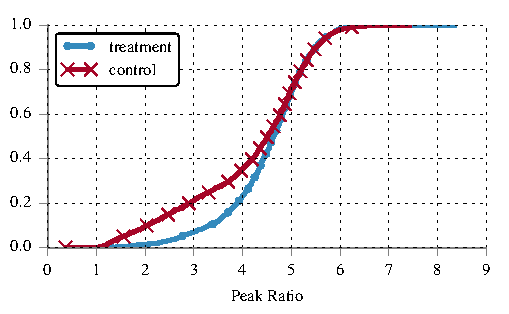
\includegraphics[width=1\linewidth]{figures/peakratio_cdf_mean-devices.pdf}
\caption{Distribution of the average peak ratio per subscriber in the treatment and 
control groups.}
\label{fig:CDF-peak-ratio-mean}
\end{minipage}
\end{figure}

Figure~\ref{fig:CDF-peak-ratio-mean} plots the peak-to-mean ratio for each 
subscriber in the treatment and control groups. The median peak-to-mean
ratio for subscribers from the treatment group is 4.64, compared to 4.51
for the control group.
\f{We found that 40\% of the subscribers in both groups have peak ratios
greater than 5; the peak-to-mean ratios 
of subscribers in the treatment group are higher than those in the
control group, perhaps indicating that users in higher service tiers do
in fact use the additional capacity for short periods of time.}

The decrease in prime-time ratio by volume, and a consistent increase in
the peak-to-mean ratio per subscriber indicates the following:
Subscribers in the treatment group have higher peak-to-mean ratio than
those in the control group. However, these subsribers tend to still have
low absolute demand, so these relative increases do not significantly
affect total traffic during prime-time and, when it is high, the demand
tends to be in non-prime-time hours.  Consistent with the results in
Section~\ref{subsec:primetime} also found that on weekdays, the
peak-to-mean ratios in the treatment group are higher than the control
group, whereas on weekends peak-to-mean ratios for both the control and
treatment groups are similar.
